
\chapter{Atividades Realizadas}
\label{cap:atividades}

  O objetivo desse capítulo é relatar as diversas atividades realizadas no 
  planejamento e desenvolvimento do Projeto Ouroboros. Explicaremos como de
  fato implementamos a solução apresentada no capítulo anterior, as
  dificuldades técnicas encontradas e todos os outros recursos que utilizamos
  para concretizar nossa ideia.

  Porém, a modelagem que fizemos até agora reflete o modo como nós enxergamos
  \emph{atualmente} nosso projeto. Como ressaltamos na introdução, já havíamos
  desenvolvido boa parte do nosso sistema bem antes do trabalho de formatura,
  e ele passou por algumas modificações desde então. Logo, como este capítulo
  descreverá as atividades que fizemos, ele adotará um fluxo mais cronológico
  dos assuntos, descrevendo o que fizemos desde o começo do sistema. Por isso,
  haverá momentos em que o que fizemos ainda não condizirá com a estrutura
  apresentada no capítulo \ref{cap:estrutura}, mas ilustrará o processo pelo
  qual passamos antes de alcançar o nosso entendimento atual do projeto e do
  domínio onde ele exerce seu papel.
  
  \section{Origem do projeto}
  \label{sec:atividades:origem}
  
    No início deste ano, elegemos para o nosso trabalho de formatura supervisionado
    o aprimoramento de um sistema que já estávamos desenvolvendo desde o começo de
    2011, como parte das nossas atividades no USPGameDev. Originalmente, ele fazia
    parte de um outro projeto do grupo chamado UGDK\footnote{A UGDK é um dos
      principais projetos do USPGameDev, e seu
      nome é um acrônimo que pode significar tanto \emph{USP Game Development
      Kit} quanto \emph{USPGameDev Kit}. Ela é desenvolvida em \CXX{}, disponível em:
      \url{http://uspgamedev.org/projetos/ugdk/} (último acesso: 26/11/2013)
    }, uma \emph{engine}\footnote{Mais informações:
      \url{http://www.gamecareerguide.com/features/529/what\_is\_a\_game\_.php}
      (último acesso: 26/11/2013)
    } de desenvolvimento de jogos digitais bidimensionais (ou
    simplesmente ``jogos 2D''). A ideia surgiu devido a uma situação com
    outro projeto, também do USPGameDev: o jogo digital chamado
    \emph{Horus Eye}\footnotemark{}. Ele era programado em \CXX{} e usava os
    recursos da UGDK para ter acesso às funcionalidade essenciais de mídia e
    interatividade que um jogo precisa. A equipe estava tendo muitas dificuldades
    em expandir o conteúdo dele desde o seu lançamento em outubro de 2010, pois
    não só apenas os membros mais antigos sabiam programar em \CXX{}, como também
    só eles sabiam \emph{o que} precisava ser mudado para obter os resultados
    desejados. A solução que propusemos foi integrar o jogo com \script{s}, pois
    assim até mesmo não programadores poderiam contribuir com o desenvolvimento
    de mais conteúdo para ele. Foi então que elaboramos o chamado ``sistema de
    \script{s} da UGDK'', que depois viria a se tornar o objeto deste trabalho.

    \footnotetext{Disponível em: \url{uspgamedev.org/horus-eye} (último acesso: 25/07/2013)}

    Ele fornecia ferramentas que buscavam simplificar o máximo possível a
    troca de dados entre o jogo e os \script{s}. Para que a elaboração de conteúdo
    novo do jogo pudesse ser programada majoritariamente através destes, bastava
    isolar as partes mais críticas daquele. Por exemplo, para um desenvolvedor de
    conteúdo não interessa saber quais rotinas devem ser evocadas para criar uma
    nova fase, mas sim como descrever as fases; então, deixávamos os \script{s}
    responsáveis por especificar a forma e os eventos de cada fase, e depois o
    código nativo do jogo cuidava de analisar esses dados e executar os
    procedimentos necessários para que a fase passasse a existir. E dessa maneira
    tornamos possível aprimorar o jogo usando linguagens bem mais simples que \CXX{}
    e sem a necessidade de conhecer todas as minúcias do seu código.

    \begin{figure}[ht]
      \centering
      \caption{}
      \begin{subfigure}{.8\textwidth}
        \begin{center}
          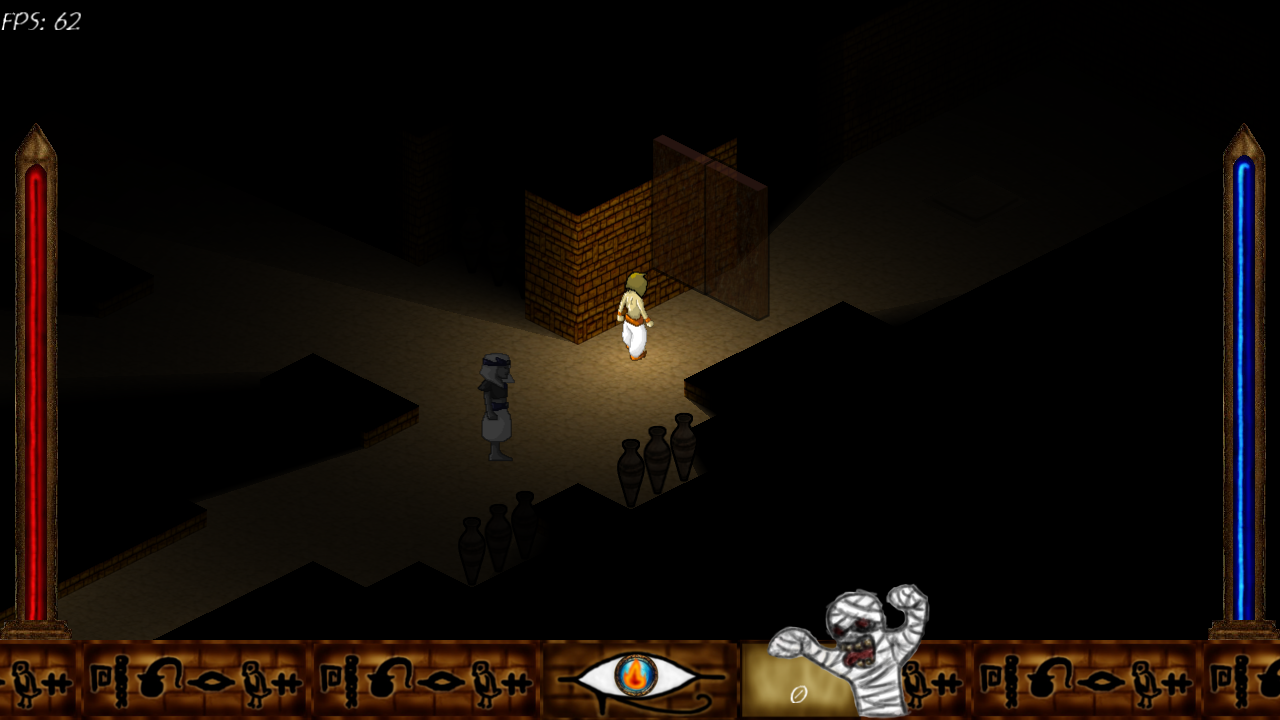
\includegraphics[width=\textwidth]{horus-2.png}
          \vspace{1em}

          \textit{
            Uma fase feita para o \emph{Horus Eye} usando o sistema de \script{s}
            da UGDK. É possível posicionar e especificar tanto elementos estáticos
            como vasos quanto elementos interativos como as portas e as múmias,
            graças às facilidades que \emph{scripting} traz ao desenvolvimento.
          }
        \end{center}
      \end{subfigure}
      \label{fig:horus}
    \end{figure}

    Comparando com a estrutura apresentada no capítulo anterior, o que tínhamos
    desenvolvido é o que hoje corresponde à OPA. A parte pela qual o OPWIG seria
    responsável era tratada por uma ferramenta à parte, sobre a qual falaremos ao
    longo das sessões que seguem. Ela é um dos principais motivos pelo qual, apesar
    de termos sido bem sucedidos em desenvolver esse sistema, ele ainda era
    razoavelmente delicado de manipular e continha várias limitações.

  \section{Decisões de projeto}
  \label{sec:actividads:decisoes}

  Antes de adentrarmos as atividades de implementação, gostaríamos de apresentar
  as decisões que adotamos para o trabalho em nosso projeto. Principalmente
  porque elas também sofreram alterações ao longo do tempo, refletindo bastante
  no que tivemos que fazer ao longo do desenvolvimento. Trataremos tanto das
  ferramentas que optamos por usar, quanto das metodologias e convenções que
  escolhemos.

  \subsection{Decisões anteriores ao Trabalho de Formatura}
  Quando começamos a desenvolver o nosso ``sistema de \script{s}'',
  como ele era integrado à UGDK e fazia parte do USPGameDev, muitas das
  nossas decisões do projeto refletiam os padrões de projeto que seguíamos
  no grupo. Segue uma relação das decisões tomadas sobre ferramentas e
  metodologias usadas. Quando necessário, daremos um resumo sobre as
  ferramentas apresentadas.

  \begin{enumerate}

    \item \textbf{Linguagens usadas}: \CXX{} para a biblioteca, \lang{Lua} e
      \lang{Python} para integração.
      \begin{itemize}
        \item[Motivo -]
          \CXX{} era a linguagem que a UGDK e os nossos
          jogos usavam. Além disso é comum linguagens de \script{} terem uma
          implementação de sua máquina virtual em \C{}, ou até \CXX{}. Ainda
          mais, como \CXX{} contém em si todas as funcionalidades de \C{},
          não temos perda técnica nenhuma em usar o primeiro ao invés do segundo.
          % Será que não já falamos disso antes?
          Também decidimos que o sistema seria generalizado para poder
          funcionar com possivelmente qualquer linguagem de \script{}, mas
          inicialmente iríamos incluir apenas compatibilidade com \lang{Lua}
          (a qual o Wilson conhece bem) e \lang{Python} (usada regularmente
          pelo Fernando).
      \end{itemize}

    \item \textbf{Compiladores}: \lang{g++}\footnote{Disponível em:
      \url{http://gcc.gnu.org} (último acesso: 28/11/2013)} em Linux e Visual
      Studio\footnote{Mais informações: \url{http://www.visualstudio.com} (último
      acesso: 22/11/2013)} 2010 em Windows.
      \begin{itemize}
        \item[Sobre -]
          O \lang{g++} é o compilador para \CXX{} do projeto GNU, e o Visual Studio
          é um ambiente de desenvolvimento para \CXX{} e algumas outras linguagens
          feito pela Microsoft para Windows, contendo uma
          IDE\footnote{\textit{Ambiente de Desenvolvimento Integrado}, do inglês,
          ``\textit{Integrated Development Environment}''},
          compilador e outras ferramentas.
        \item[Motivo -]
          No USPGameDev, cada membro é livre para usar o compilador que achar melhor,
          e os projetos evitam usar funcionalidades específicas que dificultem
          essa portabilidade.
      \end{itemize}

    \item \textbf{Compatibilidade}: Multi-plataforma com CMake\footnote{Disponível
      em: \url{http://www.cmake.org} (último acesso: 22/11/2013)}.
      \begin{itemize}
        \item[Sobre -] \textit{Software} livre para gerenciar a compilação, os testes
          e a entrega de aplicações multi-plataforma.
        \item[Motivo -] Para simplificar a compilação em diversas plataformas e
          compiladores. Além disso, apesar do nosso sistema fazer parte
          da UGDK, o usuário da \textit{engine} podia configurar ela para ser
          compilada com essa parte dela desativada (caso ele não precise integrar
          com \script{s}, por exemplo). Isso era feito através da manipulação de
          variáveis de configuração na descrição de projeto em CMake da UGDK.
      \end{itemize}

    \item \textbf{Distribuição e versionamento}: Usando um repositório
      Git\footnote{Disponível em: \url{http://git-scm.com/} (último acesso em: 22/11/2013)}
      hospedado no GitHub\footnote{Acessível em: \url{https://github.com/} (último
      acesso: 22/11/2013)}.
      \begin{itemize}
        \item[Sobre -] Git é um \textit{Software} Livre para versionamento cooperativo
          de código fonte. É possível configurar seu próprio servidor ou recorrer a um
          pronto. No caso, o GitHub fornece esse serviço de hospedagem de repositórios Git.
        \item[Motivo -] O grupo gosta de deixar as ferramentas que desenvolve à
          disposição da comunidade, para quem quiser aprender com elas. Como nosso
          sistema fazia parte do código da UGDK, ele compartilhava o repositório dela.
      \end{itemize}

    \item \textbf{Geração de \textit{wrappers}}: SWIG \cite{swig:00}.
      \begin{itemize}
        \item[Sobre -] Por extenso, seu nome é \emph{Simplified Wrapper and
          Interface Generator}, e ele essencialmente exporta código nativo
          para diversas linguagens virtuais, inclusive as que usamos. Iremos explicar
          bastante sobre como ele é usado algumas seções a frente.
        \item[Motivo -] Foi a melhor opção para o que necessitávamos segundo
          nossa pesquisa, era uma ferramenta pronta para proporcionar a
          geração de \textit{wrappers} que sabíamos que seria difícil de
          desenvolver nós mesmos a tempo de atender a demanda para o sistema
          no USPGameDev.
      \end{itemize}

    \item \textbf{Metodologia}: Uma variação própria de métodos ágeis do USPGameDev.
      \begin{itemize}
        \item[Sobre -] O trabalho de formatura de Vinicius K. Daros
          \cite{scrum:00} trata com bastante detalhes sobre as metodologias
          de trabalho do USPGameDev naquela época.
        \item[Motivo -] As metas que seguíamos nas iterações de trabalho
          estavam mescladas com as metas do jogo \textit{Horus Eye} e da
          \textit{engine} UGDK, de forma que a maior parte do que
          desenvolvíamos era voltado para ser usado nesses outros
          programas. Logo, trabalhávamos em conjunto com o resto do
          grupo usando a mesma metodologia.
      \end{itemize}

  \end{enumerate}

  \subsection{Mudanças no Projeto para o Trabalho de Formatura}
  Quando começamos o trabalho de formatura, fizemos algumas mudanças nas nossas
  decisões de projeto originais. Primeiramente, separamos o sistema para ser um
  projeto separado, totalmente independente de qualquer outro projeto do
  USPGameDev, e o nomeamos Projeto Ouroboros. Partindo do código fonte
  original, criamos outro repositório Git específico para o Ouroboros\footnotemark{},
  e também  o hospedamos no GitHub. Mantivemos o uso de CMake, pois, dentre outras
  razões, ele permitiu-nos simplificar algumas partes do nosso sistema tanto para os
  desenvolvedores quanto para os usuários (mais informações na seção
  \ref{cap:atividades:cmake}). Abaixo listamos as principais mudanças feitas
  com relação às outras decisões anteriores, assim como algumas novas que
  surgiram com a emancipação do nosso sistema.

  \footnotetext{Repositório do Projeto Ouroboros:
                \url{https://github.com/Rewasvat/ouroboros}
                (último acesso: 1/12/2013)}
  
  \begin{enumerate}

    \item \textbf{Linguagens usadas}: As mesmas, só que com um padrão mais
      recente de \CXX{} conhecido como \CXX{11}.
      \begin{itemize}
        \item[Sobre -] Nesse novo padrão, inúmeras facilidades são
          introduzidas à linguagem. As mais relevantes para nosso projeto
          foram as funcionalidades de coleta de lixo automatizada e
          os \textit{variadic templates}.
        \item[Motivo -] Além da diversas facilidades que tornaram o
          desenvolvimento do sistema mais produtivo, algumas das
          ferramentas que passamos a usar já adotavam esse novo padrão,
          e portanto achamos melhor acompanhá-las nessa iniciativa para
          evitar incompatibilidades.
      \end{itemize}

    \item \textbf{Compilador}: Apenas \lang{g++}.
      \begin{itemize}
        \item[Motivo -] O uso de \CXX{11} introduziu um problema no projeto:
          compatibilidade de compiladores com essa versão nova. Como o \CXX{11}
          ainda é razoavelmente recente, nem todos compiladores reconhecem
          todas suas novas funcionalidades. Mais notavelmente, não conseguimos
          mais compilar no Windows com o Visual Studio 2010, e nem com sua
          versão mais recente, Visual Studio 2013. No Linux, tivemos que usar
          uma versão mais nova do \lang{g++}, a 4.7. Apesar de existirem
          versões ainda mais recentes, essa era a mínima necessária.
      \end{itemize}

    \item \textbf{Gerador de \textit{wrappers}}: Abandonamos o uso de SWIG
      para substituí-lo pelo nosso próprio gerador, o OPWIG.
      \begin{itemize}
        \item[Sobre -] Já explicamos sobre ele na seção \ref{cap:estrutura:opwig}
          e falaremos sobre sua implementação na seção \ref{sec:actividads:opwig}.
        \item[Motivo -] Também trataremos dos motivos por trás desse mudança
          em outra seção, a \ref{cap:atividades:swig-sux}.
      \end{itemize}

    \item \textbf{Metodologia}: Organização das metas em \textit{milestones}.
      \begin{itemize}
        \item[Sobre -] Após separar o projeto de USPGameDev, inicialmente
          mantivemos listas de tarefas pendentes e fixávamos objetivos
          periodicamente para serem completados o quanto antes (algo vagamente
          parecido com iterações de programação ágil, porém não tão bem
          organizado). A partir do segundo semestre desse ano, adotamos o
          uso de \textit{milestones}\footnotemark{} (ou ``marcos'', em português):
          elaborávamos uma pequena aplicação de um usuário fictício do nosso
          sistema, e desenvolvíamos apenas o necessário para que a aplicação
          dele funcionasse devidamente. Após completar uma \textit{milestone},
          montávamos uma outra mais complicada e que exigisse mais do nosso
          projeto, e repetíamos o processo. Além disso, recentemente passamos
          a aproveitar algumas funcionalidades do GitHub justamente voltadas
          para o gerenciamento de tarefas que caíram muito bem com essa
          metodologia.
        \footnotetext{O uso que damos à palavra \textit{milestone} nesse trabalho
                      provavelmente não reflete exatamente o sentido usual que ela
                      tem no desenvolvimento de \textit{software}.}
        \item[Motivo -] Ao estabelecer uma meta tão clara quanto um caso de uso,
          o desenvolvimento fica muito mais produtivo e objetivo. Durante o
          primeiro semestre gastamos bastante tempo cobrindo partes do nosso
          sistema que até agora não foram completamente utilizadas. Se esse
          esforço tivesse sido melhor direcionado, provavelmente o projeto estaria
          mais adiantado. O método das \textit{milesones} ainda por cima é
          bastante compatível com os princípios de programação ágil, pois provê
          um processo iterativo que prioriza o desenvolvimento das funcionalidades
          mais críticas e relevantes ao produto.
      \end{itemize}


    \item \textbf{Testes automatiazdos}: Usando \textit{googletest}\footnote{Disponpivel
      em: \url{https://code.google.com/p/googletest/} (último acesso: 29/11/2013)} e
      fazendo integração contínua com Travis\footnote{Acessível em:
      \url{https://travis-ci.org/} (último acesso: 29/11/2013)}.
      \begin{itemize}
        \item[Sobre -] O \textit{googletest} é um arcabouço para escrever e
          executar testes automatizados em \CXX{}, desenvolvido pela Google.
          Já o Travis é um serviço de integração contínua: ele
          automaticamente clona respósitórios no GitHub quando há alguma
          modificação neles, e executa uma sequência de comandos (determinadas
          pelo dono de cada repositório) para verificar se o código do projeto
          compila com sucesso e passa nos testes especificados para ele. Para usar o
          Travis basta registrar o repositório desejado usando sua própria conta
          do GitHub, e ele irá inclusive enviar e-mails para os desenvolvedores
          sempre que algo falhar nos testes.
        \item[Motivo -] Como passamos a desenvolver nosso próprio gerador de
          \textit{wrappers}, precisávamos de uma segurança melhor sobre o
          funcionamento dele. Usar testes automatizados permitiu-nos desenvolver
          com muito mais tranquilidade, certeza e produtividade. Ao mesmo tempo,
          o uso do Travis permite que testemos nosso \textit{software} em
          um ambiente que não seja o nosso (que já está todo preparado e portanto
          seria uma referência viesada), assim como saber imediatamente quando
          algo parou de funcionar graças às notificações que ele nos envia.
      \end{itemize}
  \end{enumerate}
  
  \section{Uma interface comum para \lang{Lua} e \lang{Python}.}
  \label{sec:atividades:opa}
  Desenvolver uma interface comum entre as duas linguagens de \script{} escolhidas
  foi uma das coisas que fizemos para a UGDK, e hoje o trabalho realizado nesse
  quesito foi o que formou a OPA vista na seção \ref{cap:estrutura:opa}. Desde o
  começo vimos desenvolvendo uma interface generalizada capaz de usar uma ou outra
  máquina virtual sem diferenças na interface para o usuário. A seguir explicamos
  o que implementamos de fato nas principais classes da OPA.

  Como vimos no capítulo anterior, a princípio precisaríamos de três classes
  na nossa API: uma para representar objetos virtuais, outra para máquinas virtuais
  e a última para gerenciar essas máquinas. Mas na realidade, por questões de
  usabilidade, implementamos a classe de objetos virtuais em duas partes. Uma
  delas é a que o usuário utilizará, e portanto terá vários mecanismos facilitadores.
  A outra será a que de fato fará o trabalho sujo, escondido do usuário graças
  à primeira. Elas são as classes \VObj{} e \VData{}, respectivamente.
  
  As das máquinas virtuais e do gerenciador serão mantidas como projetamos. No
  entanto, o usuário não usará a de máquinas virtuais com tanta frequência, já a
  do gerenciador será muito mais presente e importante para ele. Principalmente
  porque o gerenciador encapsula os serviços das máquinas virtuais, então o
  acesso direto a elas torna-se desnecessário.
  
  A seguir entramos em detalhes sobre cada uma dessas classes.
  
  \subsection{\VObj{}}
  \label{sec:atividades:opa:vobj}
  Essa classe representa um objeto virtual qualquer, como explicado na seção
  \ref{cap:estrutura:opa}. É quase a única classe que o
  usuário precisa usar. Ela implementa alguns métodos que possibilitam ao
  usuário realizar sobre o tal objeto operações comuns em elementos de diversas
  linguagens de \script{}. Para tornar o uso dessa classe mais agradável, também
  sobreescrevemos alguns operadores de \CXX{} de maneira a facilitar uso de
  algumas dessas operações:
  \begin{itemize}
    \item \textbf{Executar o objeto como uma função}: simplificado pelo operador \lang{()}
      do \CXX{}, permitindo ao usuário usar as próprias instâncias de \VObj{} como
      funções. Exemplo:
      \vspace{1em}
      \begin{lstlisting}
        VirtualObj vObj, vReturnObj, vObjArg1, ..., vObjArgN; 
        VirtualObj::List vObjList; // o mesmo que std::list<VirtualObj> vObjList;
                                   // uma lista de instancias de VirtualObj.
                                   
        // Podemos evocar o objeto sem parametro nenhum
        vReturnObj = vObj();
        // Com um numero arbitrario deles
        vReturnObj = vObj( vObjArg1, vObjArg2, ... , vObjArgN );
        // Ou usando uma lista para junta-los
        vReturnObj = vObj( vObjList );
      \end{lstlisting}
    \item \textbf{Acessar e alterar atributos do objeto}: simplificado pelo operador
      \lang{[]} do \CXX{}, permitindo ao usuário usar as instâncias de \VObj{} como
      tabelas de símbolos. Exemplo:
      \vspace{1em}
      \begin{lstlisting}
        VirtualObj vObj, vAttrObj, vObj_AttrName;
        // Podemos acessar membros usando cadeias de caracteres como chave
        vAttrObj = vObj["nome_do_atributo"];
        // Ou outros objetos virtuais
        vAttrObj = vObj[ vObj_AttrName ];
      \end{lstlisting}
    \item \textbf{Executar um método do objeto (instância de uma classe)}: simplificado pelo
      operador \lang{|} do \CXX{}. Chamadas de métodos em linguagens de \script{} normalmente
      passam a instância da classe (o próprio objeto) como o primeiro argumento da
      função, e o uso desse operador com o objeto simplifica essa operação. Exemplo: 
      \vspace{1em}
      \begin{lstlisting}
        // Recebe argumentos como nas chamadas de funcao
        (vObj | "nome_do_metodo")( ... );
        // E eh equivalente a
        vObj["nome_do_metodo"](vObj, ...);
      \end{lstlisting}
    \item \textbf{Conversão de valores}: como a maioria dos métodos (e operadores) da classe
      \VObj{} recebem e devolvem instâncias dela mesma, a conversão de valores é a forma que
      fizemos para poder converter entre objetos de \CXX{} e esses objetos virtuais. Para
      tanto, a classe possui dois métodos \textit{template}\footnotemark{} que possibilitam
      a conversão de valores entre os dois ambientes. Exemplo:
      \vspace{0.5em}
      \begin{lstlisting}
        // Com ponteiros para tipos definidos pelo usuario:
        T* valor = vObj.value<T*>();
        vObj.set_value<T*>(valor);
        
        VirtualObj vNumObj; //suponha um VirtualObj contendo um numero
        double num = vNumObj.value<double>(); // pegar o valor
        vNumObj.set_value<double>(num);       // atribuir o valor
      \end{lstlisting}
  \end{itemize}

  \footnotetext{\textit{Templates} são uma funcionalidade de \CXX{} que permite
    definir parametricamente funções e classes, fazendo-as exigir um
    ou mais tipos em uma notação especial quando são usadas. Com isso,
    essas funções ou classes têm seus corpos escritos de forma generalizada
    para vários parâmetros possíveis.
    \textit{Templates} também podem receber valores aritméticos e \str{s},
    mas na interface de \VObj{}, e na maioria do nosso trabalho, somente usamos com tipos.
    Mais informações em:
    \url{http://www.cplusplus.com/doc/tutorial/templates/} (último acesso: 26/11/2013)
  }
  
  Na prática, \VObj{} é uma classe que encapsula instâncias da classe \VData{}, que veremos
  adiante, na seção \ref{sec:atividades:opa:vdata}. Todas essas operações são repassadas
  para a instância dessa última usando um padrão de código chamado \textbf{ponteiro para
  implementação}\footnotemark{}. A classe \VData{} não deve ser usada diretamente pelo
  usuário.
  
  % Wikibooks é uma boa referência?
  \footnotetext{Vide
    \url{http://en.wikibooks.org/wiki/C++\_Programming/Idioms\#Pointer\_To\_Implementation\_.28pImpl.29}
    (último acesso: 15/09/2013)
  }
  
  \subsection{\SMgr{}}
  \label{sec:atividades:opa:smgr}
  Essa é a segunda principal classe da interface comum entre linguagens, e praticamente a
  única outra classe que o usuário precisa usar além da \VObj{}. Ela segue o padrão de projeto
  \textbf{\textit{singleton}}\footnotemark{} e corresponde ao gerenciador visto na seção
  \ref{cap:estrutura:opa}. Sua responsabilidade é, portanto, gerenciar as máquinas virtuais
  que estão disponíveis no sistema, permitindo ao usuário executar algumas operações simples
  porém importantes nelas como um conjunto:

  \footnotetext{\textit{Singleton} é um padrão de projeto que permite ter
    apenas uma instância de uma classe
    num dado momento. Mais informações em \cite{patterns:00}.
  }
  
  \begin{itemize}

    \item \textbf{Inicialização e Finalização}: o gerenciador tem métodos para inicializar
      e finalizar o conjunto de máquinas virtuais. A inicialização é necessária para poder
      usá-las e também serve para
      especificar o diretório na qual \script{s} serão carregados por ele. A finalização 
      encerra a atividade das máquinas, liberando quaisquer recursos do computador que elas
      estejam usando. Exemplo:
      \vspace{0.01em}
      \begin{lstlisting}
        // SCRIPT_MANAGER() eh uma macro que fornece um ponteiro para a
        // instancia de ScriptManager.
        bool ok = SCRIPT_MANAGER()->Initialize("./caminho/para/os/scripts/");
        
        SCRIPT_MANAGER()->Finalize();
      \end{lstlisting}
      \vspace{0.5em}
      Se o valor booleano que a chamada a \lang{Initialize()} devolve for verdadeiro,
      significa que o gerenciador foi inicializado sem problemas. Caso contrário, deve
      ter ocorrido algum problema na inicialização dele.

    \item \textbf{Registro e busca de máquinas virtuais}: o gerenciador inicialmente não sabe
      quais são as máquinas virtuais disponíveis. O usuário pode tanto registrá-las manualmente com
      um simples método, quanto delegar essa responsabilidade para o código gerado pelo OPWIG, como
      veremos mais adiante. Caso ele queira, o usuário também pode buscar uma máquina
      virtual registrada. Elas são representadas no nosso sistema pela classe \VMac{},
      como veremos na próxima seção. Exemplo:
      \vspace{1em}
      \begin{lstlisting}
        //Registrando uma maquina virtual.
        VirtualMachine* vm = new python::PythonMachine();
        SCRIPT_MANAGER()->Register(vm);
        
        //Buscando uma maquina virtual.
        VirtualMachine* pyvm = SCRIPT_MANAGER()->GetMachine("Python");
        //pyvm corresponde ao mesmo vm declarado antes.
      \end{lstlisting}

    \item \textbf{Executar código de \script{}}: o gerenciador permite ao usuário tentar executar
      um código
      qualquer, dado como uma cadeia de caracteres, na máquina virtual de sua escolha. Exemplo:
      \vspace{1em}
      \begin{lstlisting}
        SCRIPT_MANAGER()->ExecuteCode("Lua", "print(42)");
      \end{lstlisting}

    \item \textbf{Carregar módulos}: possivelmente o método mais importante da classe \SMgr{},
      este método recebe um caminho para um arquivo de \script{} (sem a extensão dele).
      Ele então determina se o \script{} existe, e de acordo com a extensão do arquivo,
      qual máquina virtual deve processá-lo.
      A tal máquina virtual então carrega o \script{} e a função devolve uma instância de \VObj{}
      representando o módulo carregado de acordo com a linguagem de \script{} usada. Exemplo:
      \vspace{1em}
      \begin{lstlisting}
        VirtualObj modulo = SCRIPT_MANAGER()->LoadModule("modulo");
        VirtualObj modulo2 = SCRIPT_MANAGER()->LoadModule("pacote.subpacote.modulo");
      \end{lstlisting}

  \end{itemize}

  \subsection{\VMac{}}
  \label{sec:atividades:opa:vmac}
  A \VMac{} é uma das duas classes abstratas do sistema que devem ser implementadas para
  cada linguagem que se deseja ser compatível com a OPA, como explicado na seção
  \ref{cap:estrutura:opa} e ilustrado pela figura \ref{fig:api-classes}.
  A \VMac{} representa a máquina virtual da linguagem em si, sendo usada internamente pelo 
  gerenciador, e portanto ela raramente ela será usada diretamente pelo usuário. A figura
  \ref{fig:uml-vms} contém o diagrama UML que expressa a relação entre essas duas classes
  e também as duas implementações de máquina virtual padrão do nosso sistema. Alguns
  métodos importantes de sua interface são:
  
  \begin{itemize}
    \item Inicialização e Finalização da máquina virtual, evocadas pelo gerenciador
      no momento adequado.
    \item Método para retornar a cadeia de caracteres correspondente à extensão de um 
      arquivo de \script{} dessa linguagem.
    \item Carregar módulos, que é a operação usada internamente pelo gerenciador.
    \item Executar código \script{}, também usado pelo gerenciador.
    \item Fornecer uma nova instância vazia de \VData{} (ver próxima seção) correspondente à
      linguagem da máquina.
  \end{itemize}

  \begin{figure}[ht]
    \centering
    \caption{}
    \begin{subfigure}{.8\textwidth}
      \begin{center}
        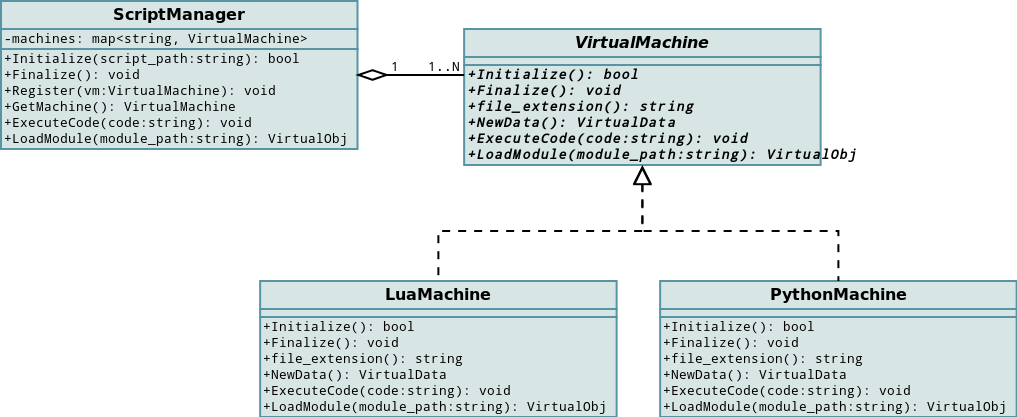
\includegraphics[width=\textwidth]{uml-vms.png}
        \vspace{1em}

        \textit{
          Os métodos apresentados correspondem às operações que destacamos para
          cada classe. A instância única de \SMgr{} armazena uma tabela que
          relaciona os nomes das linguagens de \script{} com a instância de
          máquina virtual correspondente.
        }
      \end{center}
    \end{subfigure}
    \label{fig:uml-vms}
  \end{figure}
  
  \subsection{\VData{}}
  \label{sec:atividades:opa:vdata}
  \VData{} é a segunda classe abstrata do sistema que deve ser implementada para uma linguagem
  de \script{} poder ser usada pela OPA. Ela provê os mecanismos essenciais dos objetos virtuais
  de uma linguagem específica, fornecendo todas aquelas
  operações da classe \VObj{} (descritas anteriormente). Assim, uma instância
  de \VObj{} pode ter uma instância de \VData{} implementada para uma linguagem 
  ou outra sem precisar saber qual, graças ao polimorfismo através de herança. Essa relação
  está ilustrada no diagrama UML da figura \ref{fig:uml-vdata}. Fora os métodos para as
  operações descritas na subseção \ref{sec:atividades:opa:vobj}, um ponto importante da
  interface de \VData{} é um método para fornecer a máquina virual (contida no gerenciador)
  responsável pela instância de \VData{} em questão.

  \begin{figure}[ht]
    \centering
    \caption{}
    \begin{subfigure}{.8\textwidth}
      \begin{center}
        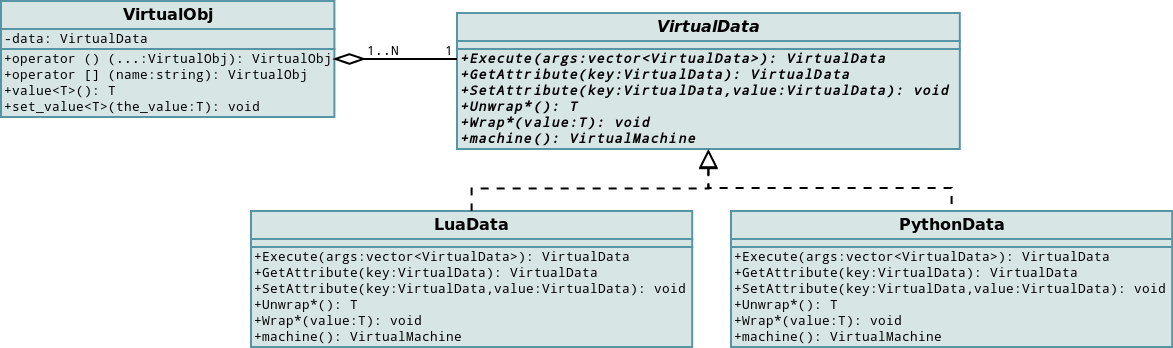
\includegraphics[width=\textwidth]{uml-vdata.png}
        \vspace{1em}

        \textit{
          Os métodos \lang{Wrap} e \lang{Unwrap} mostrados na verdade correspondem
          a uma série de métodos distintos, cada um responsável pela conversão entre
          valores nativos e virtuais de um tipo específico. Optamos por não indicar
          todos eles para simplificar o diagrama.
        }
      \end{center}
    \end{subfigure}
    \label{fig:uml-vdata}
  \end{figure}
  
  \section{Integração com SWIG}
  \label{sec:actividads:integracaoswig}
  O SWIG é uma ferramenta para exportar uma interface \C{}/\CXX{} para diversas 
  linguagens de \script{}. Um dos usos padrão dessa ferramenta (e 
  a forma como usamos) é gerar o código de \textit{wrapper} necessário para criar 
  módulos virtuais para uma máquina virtual.
  E é isso que possibilita a linguagem virtual correspondente ter acesso a uma
  interface desenvolvida em \CXX{}.
  
  A princípio, o SWIG servia para complementar nosso sistema, visto que tínhamos
  as versões antigas da OPA para permitir que a aplicação
  do usuário incorpore \script{s} mas não havíamos feito nada a respeito da exportação
  de funcionalidades da aplicação para os \script{s}. Após pesquisar possíveis soluções
  o que encontramos foi o SWIG, uma ferramenta já um tanto quanto antiga mas ainda usada
  na indústria e que fazia basicamente o que queríamos (o processo ilustrado na figura
  \ref{fig:gerador-funcionamento}).
  
  Como o SWIG é uma ferramenta já pronta, e que é executada para gerar código que será compilado
  com o código do usuário, a interação entre ele e o nosso sistema é bem simples. A principal
  parte está no fato que a OPA usa umas rotinas geradas pelo SWIG (para cada linguagem de
  \script{}) para conseguir converter instâncias de tipos nativos definidos usuário entre
  \CXX{} e as máquinas virtuais.
  
  O SWIG usa arquivos separados de extensão ``\lang{.i}'', chamados de ``arquivos de interface do 
  SWIG'', para determinar quais arquivos de \CXX{} ele irá processar, e como irá gerar o 
  \textit{wrapper} para tal código, como o seguinte:
  \vspace{1em}
  \begin{lstlisting}
  %module NOME_DO_MODULO

  %include "std_string.i"
  %include "std_vector.i"
  
  %{
  #include <src/coisas/coisa.h>
  %}

  %include <src/coisas/coisa.h>
  \end{lstlisting}
  \vspace{1em}
  
  Nesses arquivos de interface do SWIG é também possível escrever código que será incluído
  explicitamente no código gerado, ou usado internamente em algumas etapas, como por exemplo
  nas conversões de valores que passam pelos \textit{wrappers}. O segundo tipo de interação
  com o SWIG que fizemos está nesses arquivos. Usando o mecanismo de extensões do SWIG,
  desenvolvemos algumas funcionalidades com diversos objetivos nesses arquivos de interface,
  mas podemos classificá-las de dois jeitos:

  \begin{enumerate}
    \item Operações para fornecer à OPA informações sobre os tipos nativos definidos pelo
      usuário que serão exportados para as máquinas virtuais, através das estruturas de dados
      que o SWIG usa para representá-los. A OPA necessita desses dados para poder converter
      tais tipos entre a máquina virtual e o \CXX{}.
    \item Operações para mudar ou adicionar alguma funcionalidade ao \textit{wrapper}
      gerado. Elas essencialmente tentam resolver algum problema do SWIG, como
      a incapacidade de herdar tipos de \CXX{} nas linguagens de \script{}. Veremos mais
      sobre esses problemas na próxima seção.
  \end{enumerate}
  
  Aqui está um exemplo mais detalhado de um arquivo de interface do SWIG, com algumas 
  de nossas adições em uso:
  \vspace{1em}
  \begin{lstlisting}
  %module NOME_DO_MODULO

  // Inclui algumas definicoes nossas e do SWIG para simplificar este arquivo.
  %include <module/export.swig>
  %include <module/proxy.swig>
  %include <module/widetypes.swig>
  %include "std_string.i"
  %include "std_vector.i"
  
  // O codigo abaixo eh transcrito diretamente para o wrapper gerado.
  // Normalmente aproveitamos ele para incluir os cabecalhos apropriados.
  %{
  #include <src/coisas/coisa.h>
  #include <src/coisas/mais_coisa.h>
  %}

  // Se necessario, com essa(s) linha(s) voce pode fazer esse modulo referenciar 
  // outro modulo caso ele use alguma definicao nesse outro.
  %import(module="outro_modulo") <src/outras_coisas/outro.h>

  // Se necessario, com essa(s) linha(s) voce pode ignorar declaracoes em C++ para 
  // que elas nao sejam exportadas.
  %ignore coisas::CoisaEstranha;
  
  // Se necessario, com essa linha voce pode definir quais metodos e funcoes
  // que devolvem novas instancias de objetos - isso eh necessario para o controle 
  // correto da memoria, pois indica que a maquina virtual pode tomar posse do objeto
  %newobject coisas::CoisaBase::Foo;
  
  // Nao eh possivel exportar templates de C++, mas voce pode exportar uma 
  // especializacao, se necessario:
  %template(IntCoisa) coisas::CoisaVariavel<int>;

  // Se necessario, com essa linha voce pode habilitar proxies para tal 
  // classe de C++, para que ela possa ser herdada pelos scripts. Note que
  // soh isso nao eh suficiente para habilitar heranca.
  proxy_class(coisas::CoisaBase)

  // Finalmente isso informa ao SWIG o que exportar. No caso, diz para tudo no
  // arquivo indicado ser exportado, exceto se algo foi ignorado usando %ignore.
  %include <src/coisas/coisa.h>
  
  // Esse par enable/disable_disown eh essencialmente o contrario do %newobject
  // acima: eles definem que parametros de funcoes com o tipo/nome especificados
  // aqui terao sua posse roubada pelo C++. 
  // Isso serah explicado em detalhes mais adiante.
  enable_disown(coisas::CoisaBase* c)
  %include <src/coisas/mais_coisa.h>
  disable_disown(coisas::CoisaBase* c)

  // Aqui definimos quais classes que estamos exportando
  namespace coisas {
      export_class(CoisaBase)
  }

  // E confirmamos as classes exportadas, para o OPA saber converte-las
  // quando usar VirtualObj::value() e VirtualObj::set_value()
  confirm_exports(NOME_DO_MODULO)
  \end{lstlisting}
  
  
  \section{Problemas com SWIG}
  \label{cap:atividades:swig-sux}
  Ao longo do tempo em que fomos usando o SWIG notamos alguns problemas com ele, que eram
  refletidos no nosso sistema, impondo certas restrições. Alguns desses problemas conseguimos
  apaziguar com código inserido nos arquivos de interface do SWIG, como mencionado na seção
  anterior. Os problemas eram:
  
  \begin{itemize}
    \item \textbf{A determinação de posse de objetos depende da API do usuário e o design do SWIG
      não é prático para reconhecer essas especificações}.
      
      \textit{Ceder a posse} (\textit{disown}) é o ato de fazer que algum método da interface \CXX{}
      retire a posse de uma instância de uma classe \CXX{} que ele recebe como argumento vindo da
      máquina virtual. Normalmente, quando esta cria algum objeto \CXX{}, ou seja, um objeto
      na linguagem de 
      \script{} que encapsula uma instância de alguma classe \CXX{} que foi exportada, ela
      retém a posse de tal objeto. Quando ela for remover tal objeto virtual, seja 
      lá por qual razão, se ela detiver a posse dele, ela também irá remover da memória a
      instância \CXX{} encapsulada. Isso pode causar problemas se alguma parte do código nativo
      tem alguma referência para tal instância, e tenta remover ou simplesmente usar ela em algum
      momento após a máquina virtual já tê-la removido. Portanto fizemos que métodos
      da interface \CXX{} que recebem instâncias de classes e cuidam da remoção delas 
      internamente tiram da máquina virtual a posse de tal instância.
      
      A questão da posse de um objeto entre \CXX{} e uma máquina virtual é essencial ao
      problema que nosso sistema se propõe a tratar e ao nosso ver não tem como ser evitada.
      Por isso, essa complicação no SWIG é um grande obstáculo ao nosso trabalho.

    \item \textbf{O SWIG não exporta o aninhamento\footnotemark{} de classes,
      \textit{structs} e \textit{unions}, e aparentemente não pretende resolver isso tão cedo}.
      
      \footnotetext{Aninhar tais estruturas
        de \CXX{} é o ato de definir algumas delas dentro de outra delas.
      }
    \item \textbf{O SWIG não tem trata a herança de classes \CXX{} nos \script{s}}.
      
      A nossa ``solução'' para isso foi criar um sistema de \textit{proxies}\footnotemark{}: classes
      intermediárias em \CXX{} que derivam de uma classe base \lang{BaseProxy} e da classe
      \CXX{} que foi exportada e da qual queremos herdar. Essas classes \textit{proxy} contêm uma
      instância de \VObj{} encapsulando um objeto virtual que deve ser uma instância da classe em
      \script{} que herda a classe nativa em questão. Elas também implementam os métodos abstratos
      da classe base, usando o objeto virtual para repassar as chamadas dos métodos para a classe
      virtual. Fora a definição da classe \lang{BaseProxy}, e das classes \textit{proxy} para cada
      classe \CXX{} passível de ser herdada, para esse sistema funcionar foi também necessário uma
      grande parte de código adicionado nos arquivos de interface do SWIG.
      
      \footnotetext{Uma alternativa para simplificar esse processo está no nosso blog: 
        \url{http://projeto-ouroboros.blogspot.com.br/2013/07/gerador-de-proxies.html}
        (último acesso: 15/09/2013)
      }
      
    \item \textbf{O SWIG não exporta em seus \textit{wrappers} variáveis e métodos de classes com 
      modificador de acesso \textit{protected} (acessíveis somente pela classe em si e por 
      classes derivadas).} Isso decorre do fato que ele não tem suporte a herança, como mencionado
      anteriormente, mas ainda assim é um problema ao nosso ver.
    \item \textbf{Problemas com \textit{wrappers} de \lang{Lua}}:
      \begin{itemize}
        \item Uma das informações necessárias (metatabelas das classes) só pode ser obtida
          fazendo suposições sobre a implementação interna dos \textit{wrappers} de \lang{Lua}
          do SWIG. Ou seja, é preciso usar más práticas de programação para conseguir o
          acesso a esses dados.
        \item Duas funções internas dos \textit{wrappers} de \lang{Lua} do SWIG precisam ter uma
          linha de código alterada para que a solução de \textit{proxies} acima funcione.
          Tivemos que manipular o funcionamento interno do SWIG para que ele passasse a usar
          versões nossas dessas funções ao invés das originais.
      \end{itemize}
  \end{itemize}
  
  \section{Nosso próprio gerador de \emph{wrappers}}
  \label{sec:actividads:opwig}
  Boa parte do que explicamos nas seções anteriores neste capítulo foi o trabalho que realizamos
  antes do trabalho de formatura. E o principal ponto do trabalho nesse nosso último ano é
  exatamente o de substituir o SWIG por uma ferramenta própria que criamos, a fim de
  simplificar o uso e corrigir os erros listados na seção anterior. Mantivemos a OPA,
  fazendo algumas alterações para resolver erros, melhorar o sistema ou substituir as
  partes relativas ao SWIG para a nossa nova ferramenta: o nosso gerador de
  \textit{wrappers}, OPWIG, cujo papel foi descrito na seção \ref{cap:estrutura:opwig}.
  
  Atualmente, ele ainda não é capaz de substituir completamente o SWIG, mas ele já realiza algumas
  tarefas básicas importantes, como exportar funções, variáveis e classes. E continuamos
  o seu desenvolvimento em um passo constante razoável. Infelizmente não podemos ainda falar que
  já conseguimos resolver os problemas do SWIG pois como nossa ferramenta ainda está no meio
  do desenvolvimento, ainda não chegamos no ponto de ter que lidar com eles. Mais
  especificamente, ainda não chegamos em \textit{milestones} que exijam essas funcionalidades
  mais avançadas. No entanto, já conseguimos notar que pelo menos será relativamente fácil
  corrigir o problema de classes, \lang{structs} e \lang{unions} aninhadas. De fato, nosso
  gerador, ao analisar código \CXX{}, já reconhece essas declarações, só falta adaptarmos
  os \textit{wrappers} para tratá-las e testar em uma \textit{milestone} se de fato funciona.
  
  Uma vantagem presente no OPWIG que não existia no SWIG é o registro automático
  de máquinas virtuais no gerenciador, simplificando o código do usuário para usar o sistema. Esse
  registro automático funciona da seguinte maneira: cada módulo gerado pelo OPWIG contém um bloco
  de código de \textit{bootstrap} (inicialização), que é executado automaticamente
  quando o programa é carregado, dado que ele tenha sido compilado junto com o código
  de \textit{wrapper} gerado. O \textit{bootstrap} então registra a máquina virtual da
  linguagem de \script{} para a qual ele está exportando, caso ela ainda não tenha sido
  registrada, e registra o módulo de \script{} e seus sub-módulos nela. Colocamos um
  exemplo completo do que o gerador faz na seção \ref{cap:resultados:opwig}.
  
  Internamente, o OPWIG contém:
  \begin{itemize}
    \item Um analisador de código \CXX{}.
    \item Classes representando metadados de \CXX{}.
    \item Um gerador de código, que segue uma \textbf{especificação} para cada máquina virtual.
    \item O molde que uma especificação dessas deve seguir, recebendo
      os metadados com base nos quais será produxido o código que deverá ser escrito no
      arquivo gerado. Essa
      definição abstrata deve ser implementada para uma dada linguagem de \script{} para
      que o OPWIG seja capaz de gerar código de \textit{wrappers} para a máquina virtual dela.
      Novamente, nós criamos a implementação para \lang{Lua} e \lang{Python} como padrão.
  \end{itemize}
  
  \subsection{O analisador de \CXX{}}
  Um dos pontos mais importantes desse projeto, e que ocupou boa parte do nosso primeiro
  semestre em 2013, foi o desenvolvimento desse analisador. Ele é uma ferramenta que
  processa uma sequência de símbolos em uma dada linguagem, de acordo com a gramática
  dela, e gera uma estrutura de dados que representa o código analisado, e ao mesmo
  tempo verifica se ele está sintaticamente correto.
  
  No nosso caso, queremos analisar código \CXX{} e gerar metadados que representem as
  declarações feitas nele, como váriaveis, funções e classes. Esse processo passa por três etapas:
  \begin{itemize}
    \item A \textbf{análise léxica}, que consiste em transformar os caracteres do texto
      lido em símbolos 
      significativos de acordo com um conjunto de expressões regulares que eles devem satisfazer.
      Esses símbolos são chamados de \textit{tokens} ou símbolos terminais, formando a base da
      análise seguinte.
      Para facilitar a implementação dessa etapa no OPWIG, usamos o gerador de analisadores léxicos
      \textbf{Flexc++} \cite{flex:00}.
      
    \item A \textbf{análise sintática}, que seguindo a gramática da linguagem considerada, 
      descobre se os símbolos terminais fornecidos pela análise léxica formam uma expressão válida,
      como uma declaração, uma lista de parâmetros, uma definição de classe, etc.
      Para implementar essa parte, usamos o gerador de analisadores sintáticos \textbf{Bisonc++}
      \cite{bison:00}.
      
      O termo \textit{parser} significa analisador sintático, mas é comum encontrar essas duas
      primeiras etapas sendo realizadas juntas por uma mesma ferramenta. Como a análise sintática
      é o passo mais importante, usualmente tal ferramenta é simplesmente chamada de \textit{parser}.
      
    \item A \textbf{análise semântica}, que deve descobrir as implicações das expressões
      validadas pela análise sintática e tomar uma ação apropriada.
  \end{itemize}
  
  Tanto o Flexc++ quanto o Bisonc++ exigem um arquivo separado para descrever as
  especificações que eles devem seguir. No caso, nós fizemos o arquivo do primeiro
  seguindo as palavras reservadas e outro símbolos terminais da linguagem \CXX{},
  e o do segundo seguindo a gramática dela. No arquivo do Bisonc++ podemos
  especificar ações (blocos de código \CXX{}) a serem executadas quando um tipo
  expressão da gramática é reconhecido. Nós programamos tais ações para criar
  metadados que representam as declarações do código \CXX{} analisado,
  dando ínicio à análise semântica.
  
  \subsection{Metadados de \CXX{}}
  Esses metadados são representados por um conjunto de classes no OPWIG, indicando a estrutura e as
  declarações de código \CXX{} encontrados na análise anterior. No momento, temos dois principais
  tipos de metadados:
  \begin{itemize}
    \item Metadados de objetos normais: váriaveis, funções e enumerações.
    \item Metadados de escopos: classes e \textit{namespaces}, que além de seus atributos próprios
      também contêm outros metadados aninhados, inclusive outros escopos.
  \end{itemize}
  
  Mas esses metadados por si só não realizam nada, eles simplesmente contêm dados. O OPWIG constrói 
  eles usando o analisador, e consome eles para gerar o código correto dos \textit{wrappers}.
  
  \subsection{Especificação de \textit{wrappers}}
  \label{cap:atividades:opwig:wrappers}

  O gerador de código, junto com a especificação de \textit{wrappers} para uma linguagem
  de \script{}, transforma os metadados em um arquivo de código \CXX{} contendo os
  \textit{wrappers} que possibilitarão que o código analisado seja exportado. O que o
  gerador faz é razoavelmente simples: ele cria o arquivo de \textit{wrappers} seguindo
  um conjunto de blocos ordenados que são gerados combinando os critérios
  internos do OPWIG com a especificação para linguagem de \script{} envolvida:
  \begin{enumerate}
    \item \textbf{Inicial}: fornecido pela especificação usada, esse bloco deve conter
      definições comuns para os \textit{wrappers} no resto do arquivo.
    \item \textbf{Dependências}: fornecido pelo próprio gerador, esse bloco contém o código
      que inclui os arquivos de cabeçalho que foram analisados para criar cada módulo.
    \item \textbf{Intermediário}: fornecido pela especificação usada, esse bloco é similar ao 
      inicial, mas é posicionado após o código das dependências. Assim, se necessário,
      o desenvolvedor pode introduzir código tanto antes quanto depois das inclusões de cabeçalhos.
    \item \textbf{Metadados}: construído pela especificação usada, esse bloco na verdade é
      composto por uma sequência de sub-blocos, relativos aos \textit{wrappers} de cada
      metadado. Quando estes são normais, gera-se apenas um sub-bloco na sequência, enquanto
      que quando eles são de escopo, outra subsequência de blocos é formada: primeiro um
      bloco para marcar o começo do escopo, depois vários para os metadados contidos
      nele (com possivelmente mais escopos), e um último para marcar o final do
      escopo. No final, temos todos os \textit{wrappers} necessários para exportar
      as definições que os metadados representam.
    \item \textbf{Final}: construído pela especificação usada, esse bloco deve conter
      todo o código necessário para exportar os módulos para a máquina virtual em questão.
      Normalmente isso inclui tabelas das rotinas e das classes exportadas e a
      função de inicialização (aquelas vistas na seção \ref{cap:conceitos:apis}) de
      cada módulo virtual envolvido.
    \item \textbf{\textit{Bootstrap}}: fornecido pelo gerador de código, esse
      bloco é responsável por registrar a máquina virtual da linguagem d
      \script{} no gerenciador da OPA, caso ela ainda não tenha sido, e exportar
      para ela os módulos virtuais formados a partir dos \textit{wrapers}.
  \end{enumerate}
  

  \section{Funções auxiliares de CMake}
  \label{cap:atividades:cmake}
  
    Como dissemos na seção \ref{cap:estrutura:opwig}, a geração dos
    \textit{wrappers} precisa ser feita antes da compilação da aplicação do
    usuário pelos geradores responsáveis por tratar cada máquina virtual usada.
    Isso gera uma complicação para o usuário e outra para os desenvolvedores. A
    do lado do usuário é que ele precisa lembrar de re-gerar os
    \textit{wrappers} sempre que ocorrer alguma alteração relevante no código
    fonte de sua aplicação. E no lado dos desenvolvedores, sempre que for
    implementada a compatibilidade com uma nova máquina virtual de linguagem de
    \script{}, eles precisam compilar o executável do gerador correspondente também,
    e o código fonte deste é sempre praticamente o mesmo independentemente da máquina
    virtual usada, pois tudo que ele faz é chamar algumas rotinas da nossa biblioteca
    principal. Para facilitar esses dois procedimentos, fizemos algumas funções em
    CMake que automatizam eles. A única restrição dessa nossa solução é que o usuário teria
    que usar CMake para gerenciar a compilação da aplicação dele também. Sinceramente,
    é uma ferramenta muito útil e aceita por desenvolvedores, além de compatível com
    diversos ambientes de desenvolvimento, então lhe seria vantajoso usá-la.
    
    Enfim, para a geração de \textit{wrappers} do usuário, fizemos a função
    \lang{ouroboros\_wrap\_module()}. Basicamente, ele deve usá-la para cada módulo
    da aplicação que ele quiser exportar, especificando o nome do módulo, a
    máquina virtual para qual exportar, o diretório onde os arquivos gerados
    devem ficar e a lista de cabeçalhos que o gerador precisa analisar para formar
    o módulo. A função por sua vez fornece ao usuário o nome do arquivo que
    será gerado para que ele o inclua entre os arquivos que farão parte da
    compilação da sua aplicação. Um exemplo de uso é:

    \vspace{1em}
    
  \begin{lstlisting}[language=python]
    ouroboros_wrap_module (
      my_module                     # nome do modulo
      lua                           # linguagem para qual exportar
      src/                          # diretorio de saida
      MY_PROJECT_LUA_GENERATED_SRC  # variavel que receberah o resultado
    )
  \end{lstlisting}

    \vspace{1em}
    
    Para automatizar o processo de fazer o executável do gerador de
    \textit{wrappers} para as máquinas virtuais, fizemos uma função chamada
    \lang{ouroboros\_generate\_opwig()}. Dada a linguagem de \script{} da
    máquina virtual em questão e a classe de especificação de \textit{wrappers}
    apropriada, essa função gera o código do gerador apropriado (sim, nós geramos o
    gerador). Com isso, o desenvolvedor precisa apenas fazer seu trabalho no
    código fonte da \lang{libouroboros} e deixar que o CMake providencie o
    gerador. O código que ele precisa colocar nas suas listas de CMake é algo
    equivalente a:

    \vspace{1em}
    
  \begin{lstlisting}[language=python]
    ouroboros_generate_opwig (
      lua                                   # nome da linguagem
      languages/lua/wrapperspecification.h  # cabecalho com a especificacao
      opa::lua::WrapperSpecification        # classe que implementa especificao
    )
  \end{lstlisting}

